\documentclass[11pt,a4paper]{article}
\usepackage[spanish,es-tabla,es-nodecimaldot]{babel}
\usepackage[utf8]{inputenc}
\usepackage[T1]{fontenc}
\usepackage{lmodern}
\usepackage[margin=2.3cm,headheight=14pt]{geometry}
\usepackage{xcolor,graphicx,booktabs,tabularx,array,fancyhdr,titlesec,caption,enumitem}
\usepackage[most]{tcolorbox}
\usepackage[hidelinks]{hyperref}
\usepackage{microtype}

% Estado de la anotación humana. \kappatrue solo cuando las hojas ciegas estén
% anotadas por los dos integrantes y src/07_kappa.py haya dado la cifra real.
\newif\ifkappa
\kappafalse

\definecolor{verde}{HTML}{0B5A3C}
\definecolor{dorado}{HTML}{C8963E}
\newcommand{\pend}[1]{\textcolor{dorado}{\textbf{[#1]}}}

\titleformat{\section}{\large\bfseries\color{verde}}{\thesection.}{0.6em}{}[{\color{verde}\titlerule}]
\titleformat{\subsection}{\normalsize\bfseries\color{verde}}{\thesubsection}{0.6em}{}
\titlespacing*{\section}{0pt}{1.1em}{0.6em}
\titlespacing*{\subsection}{0pt}{0.8em}{0.3em}
\captionsetup{font=small,labelfont=bf,skip=4pt}
\setlist{nosep,leftmargin=1.4em}
\setlength{\parskip}{0.25em}

\pagestyle{fancy}
\fancyhf{}
\fancyhead[L]{\small\color{gray}Machine Learning II $\cdot$ Entrega final}
\fancyhead[R]{\small\color{gray}Universidad Externado de Colombia}
\fancyfoot[C]{\small\thepage}
\renewcommand{\headrulewidth}{0.4pt}

\begin{document}

% --------------------------------- portada
\begin{titlepage}
\centering
\vspace*{1.5cm}
{\color{verde}\rule{\linewidth}{1.5pt}}\\[0.5em]
{\scshape\color{verde}Universidad Externado de Colombia}\\[0.2em]
{\small\color{gray}Departamento de Matemáticas\\Ciencia de Datos}\\[0.3em]
{\color{verde}\rule{\linewidth}{0.5pt}}
\vspace{3cm}

{\large\bfseries\color{verde}Proyecto Integrador de Machine Learning II}\\[1.2em]
{\LARGE\bfseries Análisis de sentimiento en reseñas de\\[0.2em] banca digital colombiana}\\[1em]
{\itshape Reproducción y adaptación crítica de un protocolo comparativo\\ de clasificación supervisada de texto}\\[1.5em]
{\color{dorado}\rule{0.45\linewidth}{1pt}}\\[1.5em]
{\bfseries ENTREGA FINAL}\\[0.3em]
Fase 3: consolidación, despliegue y comunicación
\vfill
{\bfseries\color{verde}Integrantes}\\[0.5em]
Miguel Ángel Melo\\[0.3em]
Nicolás Mateo Corzo\\[1.5em]
\textbf{Asignatura:} Machine Learning II\\[0.4em]
\textbf{Repositorio:} \url{https://github.com/melo11miguel/ml2-sentimiento-banca-digital}\\[1cm]
{\color{verde}\rule{\linewidth}{1.5pt}}
\end{titlepage}

% --------------------------------- resumen
\begin{tcolorbox}[colback=verde!6,colframe=verde,title=\textbf{Resumen de la entrega},fonttitle=\small,fontupper=\small]
Cerramos el flujo con una prueba que el artículo base no tiene: 291 reseñas de Nequi, DaviPlata y Nu
publicadas entre el 30 de octubre y el 11 de noviembre de 2026, posteriores a todo el entrenamiento
y con la distribución natural de clases. El modelo final, una regresión logística sobre n-gramas de
caracteres con ponderación de clases, entrenada con oro y etiqueta débil y con los nombres de las
entidades enmascarados, obtiene en esa prueba un F1 macro de 0,889 (IC del 95\,\%: 0,83 a 0,94) y
recupera 20 de los 26 conflictos. El protocolo del artículo, aplicado a los mismos datos, alcanza su
misma exactitud (0,89) pero detecta solo 2 conflictos. SHAP muestra que el modelo reconoce el
conflicto casi siempre por el conector ``pero''. Lo desplegamos en una aplicación de Streamlit que
explica cada predicción. La limitación principal es que todas las etiquetas son preetiquetas
asistidas por IA\ifkappa\ revisadas por el equipo\else\ sin revisión humana completa\fi.
\end{tcolorbox}

\section{Modelo final y reproducción del método}

\subsection{Qué cerramos desde la Entrega 2}
La Entrega 2 dejó tres tareas que condicionaban la elección del modelo. Primero, construimos el
\textbf{conjunto de prueba temporal}: con el mismo procedimiento extrajimos las 11\,813 reseñas
publicadas entre el 1 de octubre y el 11 de noviembre de 2026; tras las mismas reglas de depuración
y tras quitar los textos que ya estaban en el corpus quedaron 6\,779, de las que tomamos 200 al azar
por entidad sin estratificar por estrellas. Las 600 se preetiquetaron con la misma guía, leyendo
solo el texto, y descartamos 19 irrelevantes (entre ellas, algunas de México que el filtro no detectó y dos en portugués). El
conflicto pesa allí el 10,5\,\%, cerca de lo que esperábamos para la distribución natural. Segundo,
\textbf{enmascaramos las entidades}: ``nequi'', ``daviplata'', ``david plata'', ``nu'', ``nubank''
y sus variantes pasan a un mismo símbolo dentro de la normalización, para que el modelo no aprenda
que mencionar Nu es señal de elogio. Tercero, decidimos con datos \textbf{si conservar la etiqueta
débil}.

Para no usar la prueba dos veces, partimos la muestra temporal por su fecha mediana. Las 290 reseñas
de octubre forman una \textbf{validación temporal} que responde solo la tercera pregunta, y las 291
siguientes son la \textbf{prueba final}, que usamos una vez. Dejamos esa regla escrita en el código
antes de ver un solo resultado.

\subsection{Selección y configuración definitiva}
La CV anidada de la Entrega 2 (Tabla~\ref{tab:anidada}) eligió la familia: la regresión logística
sobre caracteres tuvo el mayor F1 macro sobre el oro, con el bucle interno eligiendo $C=0{,}3$ en 4
de 5 pliegues; el stacking quedó empatado dentro de una desviación estándar, pero tarda casi tres
veces más y no se interpreta directamente, y CatBoost fue el árbol más estable. Con ese desempeño
equivalente, el criterio de interpretabilidad y costo inclina la decisión hacia la regresión
logística.

\begin{table}[h]
\centering\small
\caption{Validación cruzada anidada sobre el corpus de modelado (5 pliegues externos y 3 internos;
F1 sobre la muestra anotada). Selección de la familia de modelos, tomada de la Entrega 2.}\label{tab:anidada}
\begin{tabular}{lccc}
\toprule
Modelo & F1 macro & F1 conflicto & Minutos \\
\midrule
\textbf{Regresión logística (caracteres)} & \textbf{0,724 $\pm$ 0,035} & 0,686 & 2,9 \\
Stacking (LR, SVM, LightGBM) & 0,718 $\pm$ 0,037 & 0,688 & 8,1 \\
CatBoost & 0,687 $\pm$ 0,014 & 0,692 & 5,4 \\
XGBoost & 0,654 $\pm$ 0,023 & 0,579 & 8,6 \\
SVM lineal & 0,638 $\pm$ 0,032 & 0,436 & 3,8 \\
Random Forest & 0,553 $\pm$ 0,024 & 0,231 & 6,2 \\
Reg. logística por defecto (línea base) & 0,475 $\pm$ 0,024 & 0,000 & 0,2 \\
\bottomrule
\end{tabular}
\end{table}

La validación temporal invirtió lo que sugería la ablación de la Entrega 2. Allí, sobre el oro,
entrenar solo con las reseñas anotadas era mejor (0,770 frente a 0,729). En la validación temporal
pasa lo contrario: solo oro obtiene 0,790, oro y débil con peso 0,3 obtiene 0,831 y oro y débil con
el mismo peso obtiene 0,840. La explicación es la que anticipamos: el oro contiene todas las
reseñas de tres estrellas, ambiguas y dominadas por quejas, mientras que en el uso real el 46\,\% de
las reseñas son de cinco estrellas y el 36\,\% de una, justo donde la etiqueta débil acierta y aporta
volumen. Por eso la \textbf{configuración definitiva} es: normalización y enmascaramiento de
entidades, TF-IDF de n-gramas de caracteres de 2 a 5 dentro de palabra (escala sublineal, mínimo 2
documentos, máximo 60\,000 términos), regresión logística multinomial con ponderación de clases y
$C=0{,}3$ (elegido por CV interna), entrenada con las 18\,495 reseñas del conjunto de modelado.

\subsection{Evaluación en la prueba temporal}
En la prueba, el modelo final obtiene un F1 macro de 0,889 (IC del 95\,\% por bootstrap: 0,83 a
0,94) y un F1 de 0,78 en conflicto, con precisión de 0,80 y exhaustividad de 0,77 (Figura~\ref{fig:prueba}).
El stacking queda en 0,896, pero la diferencia pareada con el modelo final va de $-0{,}03$ a
$0{,}04$: no es distinguible y no justifica un modelo 18 veces más lento. CatBoost baja a 0,839
porque pierde la mitad de los conflictos. Las líneas base marcan el piso: la regresión logística por
defecto llega a 0,619 y el clasificador de mayoría a 0,214. Enmascarar las entidades no costó nada
medible: sin máscara el F1 macro es 0,892, con una diferencia de 0 a 0,008.

\begin{figure}[h]
\centering
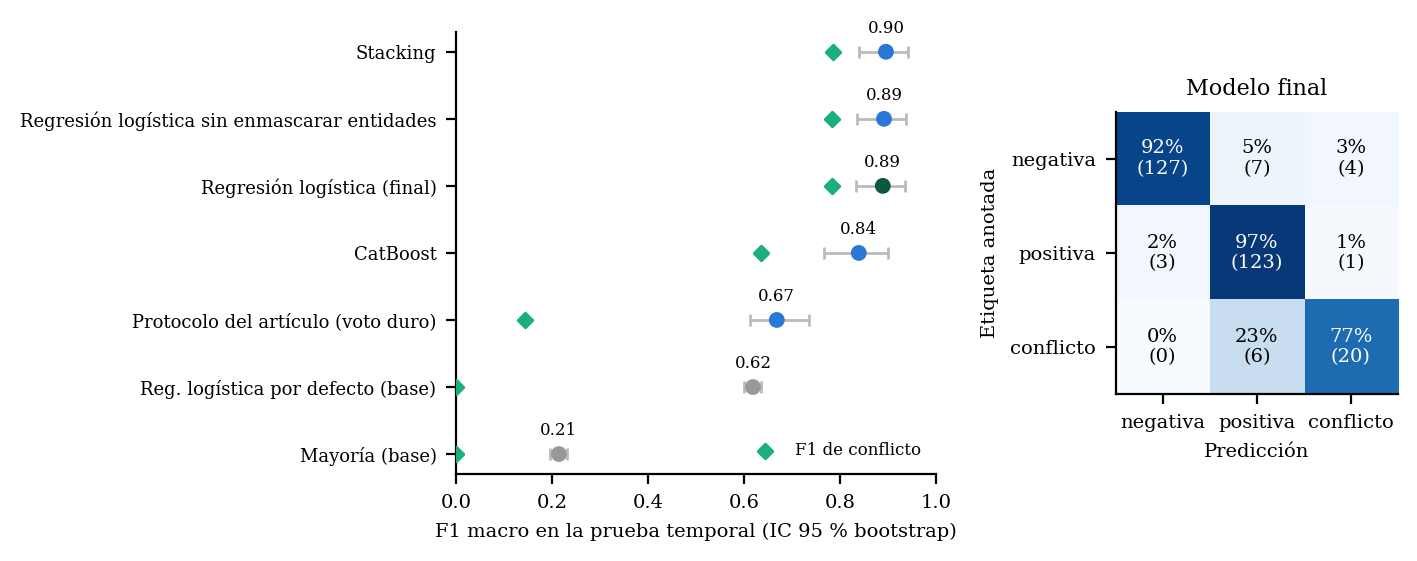
\includegraphics[width=\linewidth]{../reports/figures/fig7_prueba_temporal.png}
\caption{Prueba temporal (291 reseñas del 30 de octubre al 11 de noviembre de 2026, nunca vistas).
Izquierda: F1 macro con su intervalo del 95\,\% por bootstrap y F1 de la clase conflicto (rombos).
Derecha: matriz de confusión del modelo final (porcentaje por fila y conteo).}
\label{fig:prueba}
\end{figure}

Las cifras superan a las de la CV anidada (0,724) por la misma razón de la sección anterior: la
prueba tiene la mezcla real de reseñas, con muchas quejas y elogios inequívocos, y no la
sobrerrepresentación de casos ambiguos del oro. La lectura correcta es que el desempeño en uso real
ronda 0,89 y el de los casos difíciles ronda 0,72.

\subsection{Contraste con el método y los objetivos del artículo}
El objetivo de Alawaji y Aloraini \cite{alawaji} era comparar familias de clasificadores clásicos
sobre TF-IDF para predecir tres polaridades con una clase conflicto. Lo reprodujimos y lo
adaptamos (Tabla~\ref{tab:contraste}). Aplicado sin cambios a nuestra prueba, su protocolo alcanza
una exactitud de 0,894, prácticamente su 0,90, pero un F1 de conflicto de 0,14: reconoce 2 de 26.
Es decir, reproducimos su resultado y también su punto ciego, porque una exactitud alta se
consigue sin resolver la clase que justifica el problema. Confirmamos dos hallazgos suyos: la
ponderación de clases es indispensable (sin ella, el conflicto tiene F1 nulo) y los modelos
lineales sobre TF-IDF compiten con los ensambles. Dos decisiones suyas no se sostienen en nuestro
contexto: eliminar palabras vacías borra ``pero'', ``no'' y ``solo'', que son las señales más
fuertes del conflicto y de la negación, y el voto por mayoría no mejora la clase minoritaria.

\begin{table}[h]
\centering\small
\caption{Contraste entre el artículo base y nuestra reproducción adaptada.}\label{tab:contraste}
\begin{tabularx}{\linewidth}{>{\raggedright\arraybackslash}p{3.1cm}>{\raggedright\arraybackslash}X>{\raggedright\arraybackslash}X}
\toprule
Aspecto & Artículo (Arabia Saudita) & Nuestro proyecto (Colombia) \\
\midrule
Mejor modelo & Voto con ponderación, exactitud 0,90 & Regresión logística sobre caracteres, F1 macro 0,889 en prueba temporal \\
Su protocolo, en nuestros datos & (no aplica) & Exactitud 0,894; F1 de conflicto 0,14 \\
Clase conflicto & No se reporta por separado & F1 0,78; recupera 20 de 26 \\
Palabras vacías & Se eliminan & Se conservan: ``pero'' es la señal principal del conflicto \\
Validación & CV de 5 pliegues, sin prueba aparte & CV anidada, validación y prueba temporales, sin fuga \\
Interpretabilidad & Ninguna & SHAP por palabra, global y por reseña \\
\bottomrule
\end{tabularx}
\end{table}

\section{Interpretación de resultados}
Para leer un modelo que trabaja con fragmentos de caracteres usamos SHAP sobre el texto
\cite{shap}: el explicador quita palabras completas y mide cuánto cambia la probabilidad de cada
clase, de modo que los aportes de las palabras y la probabilidad base suman exactamente la
predicción. Lo aplicamos a las 291 reseñas de la prueba y promediamos el aporte de cada palabra que
aparece al menos cinco veces (Figura~\ref{fig:shapglobal}).

\begin{figure}[h]
\centering
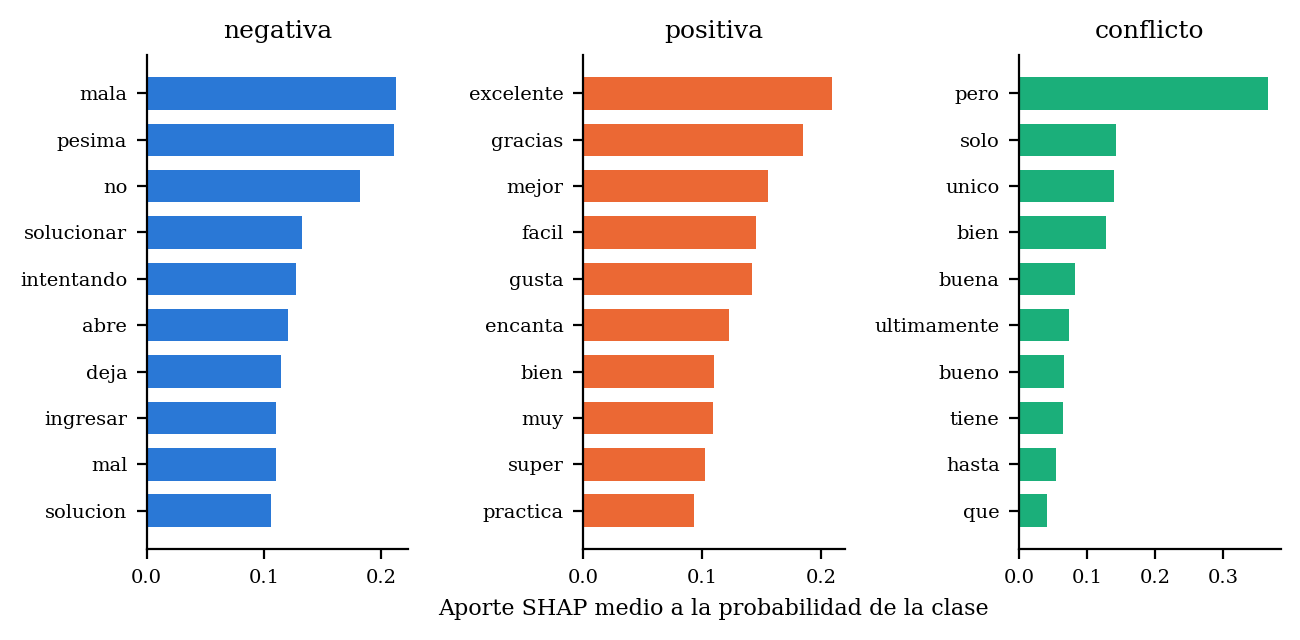
\includegraphics[width=0.86\linewidth]{../reports/figures/fig8_shap_global.png}
\caption{Diez palabras con mayor aporte SHAP medio a cada clase en la prueba temporal (palabras con
al menos cinco apariciones).}
\label{fig:shapglobal}
\end{figure}

Las tres clases se apoyan en vocabulario con sentido para el negocio. La negativa se define por
adjetivos de rechazo (``mala'', ``pésima'') y, sobre todo, por la imposibilidad de entrar: ``no''
aparece en 134 reseñas, y ``abre'', ``deja'', ``ingresar'', ``intentando'' y ``solucionar'' describen
la falla de acceso que dominó el periodo. La positiva se define por elogios y agradecimiento
(``excelente'', ``gracias'', ``fácil''). El conflicto depende casi por completo de ``pero'', con un
aporte medio de 0,37, más del doble que cualquier otra palabra, seguido de los atenuantes ``solo''
y ``único'' (``lo único malo es...'') y de los elogios tibios ``bien'' y ``buena''. El modelo
aprendió la forma retórica del conflicto: un elogio moderado seguido de una restricción.

Esa misma regla explica los errores (Figura~\ref{fig:shaplocal}). De los 26 conflictos, los 6
perdidos se leyeron como positivos: son reseñas con un elogio fuerte (``excelente'' aporta +0,31) y
una queja sin conector de contraste. De las 138 negativas, 7 se leyeron como positivas, por dos
causas principales: una negación que el modelo no capta (``no estoy feliz'', ``no me está funcionando bien'') y
saludos que confunde con elogios (``buenas'' aporta +0,42 en una queja). Y la única positiva leída
como conflicto usa ``pero'' como intensificador (``sencilla, pero sobre todo paciente''). Las
entidades ya no son señal por su nombre, aunque el símbolo enmascarado conserva algo de peso:
mencionar a la entidad, cualquiera que sea, es más común en elogios (aporta +0,06 a positiva en 46 reseñas). Por entidad, el F1 macro es de
0,89 en Nequi, 0,86 en Nu y 0,74 en DaviPlata; esta última cifra refleja que en su prueba casi no
hay reseñas positivas, no que el modelo falle en sus quejas (exactitud de 0,95).

\begin{figure}[h]
\centering
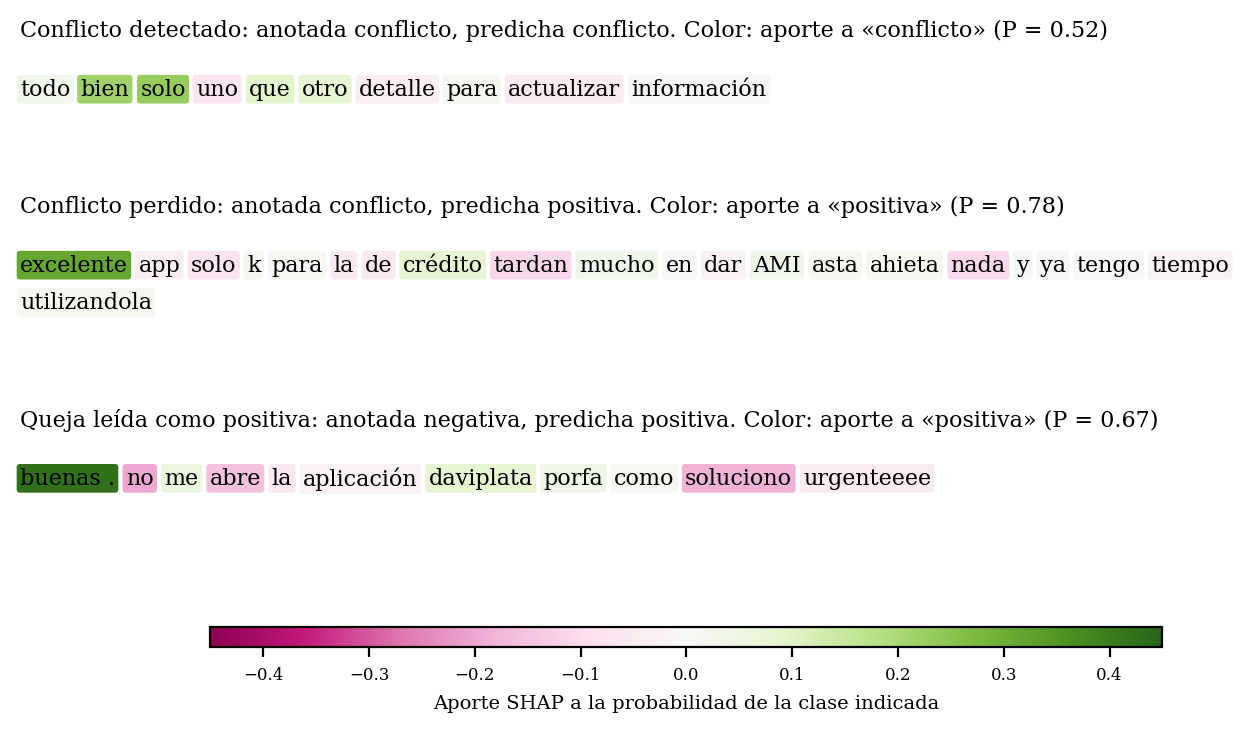
\includegraphics[width=0.86\linewidth]{../reports/figures/fig9_shap_local.png}
\caption{Explicaciones SHAP de tres reseñas de la prueba. Cada palabra se colorea según su aporte a
la clase indicada en el título: verde sube la probabilidad y morado la baja.}
\label{fig:shaplocal}
\end{figure}

En términos prácticos, el modelo sirve para \textbf{priorizar reseñas de conflicto}: de cada cinco
que marca, cuatro lo son, y encuentra tres de cada cuatro. Esas reseñas son las más valiosas para
una entidad, porque vienen de usuarios que valoran el servicio pero señalan una falla concreta y
corregible. El tipo de error también orienta el uso: rara vez inventa un conflicto (solo 5 de las 25
reseñas que marca como conflicto no lo son), y los conflictos que pierde se van hacia la clase
positiva, nunca hacia la negativa. El costo principal es
dejar pasar algunas quejas suaves envueltas en elogios, no inventar alarmas.

\section{Despliegue básico}
Desplegamos el modelo en una aplicación de Streamlit (\texttt{app/app.py}). Recibe una reseña
escrita tal como la publicaría un usuario, devuelve la clase y la probabilidad de cada una, y
explica la predicción coloreando cada palabra según su aporte SHAP; también procesa un archivo CSV
con una columna \texttt{texto} y permite descargar los resultados. La barra lateral resume el
desempeño en la prueba temporal y advierte que es un instrumento de monitoreo y no un clasificador
autónomo.

La coherencia entre entrenamiento y uso está garantizada por construcción y verificada. El archivo
\texttt{models/modelo\_final.joblib} contiene un único \texttt{Pipeline} que incluye la
normalización y el enmascaramiento, de modo que la aplicación no reimplementa ningún paso. Al
guardarlo, el script comprueba que sus predicciones sobre el texto crudo de las 291 reseñas de
prueba son idénticas a las del modelo evaluado, y el proceso se detiene si alguna difiere. También
probamos la aplicación de forma automática con \texttt{streamlit.testing} (carga, clasificación,
explicación y aviso ante un texto vacío). Se ejecuta con
\texttt{.venv/bin/streamlit run app/app.py} tras instalar \texttt{requirements.txt}, como describe
el README del repositorio.

\section{Calidad, limitaciones y proyección}
\textbf{Etiquetas.} Es la limitación principal.
\ifkappa
\pend{completar con el kappa real de las hojas ciegas}
\else
Todas las etiquetas de oro, las de entrenamiento y las de la prueba, son preetiquetas asistidas por
IA con la misma guía escrita, y no completamos la revisión humana ni el cálculo del kappa entre
anotadores. Esto tiene una consecuencia concreta: el desempeño medido es el acuerdo del modelo con
un criterio aplicado de forma consistente, y una anotación humana, con su propio desacuerdo
interno, probablemente lo bajaría. Las hojas ciegas y el script del kappa están listos en el
repositorio para cerrar esta brecha.
\fi
No usamos simulación; el supuesto análogo es la etiqueta débil por estrellas, cuyo error medimos en
16,8\,\%.

\textbf{Tamaño y alcance de la prueba.} La prueba tiene 291 reseñas y solo 26 conflictos, por lo que
el F1 de esa clase es impreciso (un acierto más o menos lo mueve cerca de 0,04), y cubre seis semanas
dominadas por fallas de acceso tras actualizaciones. Las conclusiones se refieren a quienes escriben
reseñas en Google Play, no al conjunto de los clientes. El riesgo de sobreajuste es bajo, porque la
familia se eligió con CV anidada, la variante con una validación separada y la prueba se usó una
sola vez, aunque la decisión sobre la etiqueta débil se tomó con 290 reseñas.

\textbf{Límites del modelo.} Una bolsa de n-gramas no representa el orden ni el alcance de la
negación, y por eso falla con ``no estoy feliz'', con el contraste implícito (``funcionaba de
maravilla, desde la actualización no abre'') y con el ``pero'' intensificador.

\textbf{Proyección.} En \textit{Deep Learning}, el siguiente paso es ajustar un modelo de lenguaje
preentrenado en español, como BETO \cite{beto}, cuyas representaciones contextuales sí capturan la
negación y el contraste sin conector; nuestra prueba temporal y nuestras líneas base sirven como
referencia para medir si ese costo adicional se justifica. En \textit{MLOps}, el modelo necesita un
ciclo de vida: vigilar cada semana la distribución de predicciones y el vocabulario nuevo (cada
actualización de una aplicación cambia de qué se queja la gente), anotar una pequeña muestra
periódica eligiendo las reseñas con mayor incertidumbre (aprendizaje activo), registrar y versionar
cada modelo con sus métricas, y reentrenar con integración continua cuando el desempeño caiga.

\section*{Anexo: código y declaración de uso de IA}
\small
Repositorio público: \url{https://github.com/melo11miguel/ml2-sentimiento-banca-digital}. El
archivo \texttt{run\_all.sh} reproduce todo el flujo con semilla 42 a partir de los corpus congelados
y anonimizados de \texttt{data/raw}. Usamos Claude (Anthropic) como apoyo en la escritura de
código, el preetiquetado de las dos muestras anotadas y la revisión de redacción. Todas las
decisiones metodológicas fueron discutidas y son sustentables por ambos integrantes.

\begin{thebibliography}{9}\small
\bibitem{alawaji} Alawaji, R. y Aloraini, A. (2025). Sentiment Analysis of Digital Banking
Reviews Using Machine Learning and Large Language Models. \textit{Electronics}, 14(11), 2125.
\url{https://doi.org/10.3390/electronics14112125}
\bibitem{shap} Lundberg, S. M. y Lee, S.-I. (2017). A Unified Approach to Interpreting Model
Predictions. En \textit{Advances in Neural Information Processing Systems}, 30.
\bibitem{cawley} Cawley, G. C. y Talbot, N. L. C. (2010). On Over-fitting in Model Selection and
Subsequent Selection Bias in Performance Evaluation. \textit{JMLR}, 11, 2079-2107.
\bibitem{beto} Cañete, J., Chaperon, G., Fuentes, R., Ho, J.-H., Kang, H. y Pérez, J. (2020).
Spanish Pre-Trained BERT Model and Evaluation Data. \textit{PML4DC at ICLR 2020}.
\bibitem{sklearn} Pedregosa, F. et al. (2011). Scikit-learn: Machine Learning in Python.
\textit{JMLR}, 12, 2825-2830.
\end{thebibliography}
\end{document}
